\documentclass[10pt,mathserif]{beamer}

\usepackage{graphicx,amsmath,amssymb,tikz,psfrag}

% ------------------------------------------------------------------------
% Packages
% ------------------------------------------------------------------------
\usepackage{amsmath}
\usepackage{tabularx}

% ------------------------------------------------------------------------
% Macros
% ------------------------------------------------------------------------
%~~~~~~~~~~~~~~~
% List shorthand
%~~~~~~~~~~~~~~~
\newcommand{\BIT}{\begin{itemize}}
\newcommand{\EIT}{\end{itemize}}
\newcommand{\BNUM}{\begin{enumerate}}
\newcommand{\ENUM}{\end{enumerate}}
%~~~~~~~~~~~~~~~
% Text with quads around it
%~~~~~~~~~~~~~~~
\newcommand{\qtext}[1]{\quad\text{#1}\quad}
%~~~~~~~~~~~~~~~
% Shorthand for math formatting
%~~~~~~~~~~~~~~~
\newcommand\mbb[1]{\mathbb{#1}}
\newcommand\mbf[1]{\mathbf{#1}}
\def\mc#1{\mathcal{#1}}
\def\mrm#1{\mathrm{#1}}
%~~~~~~~~~~~~~~~
% Common sets
%~~~~~~~~~~~~~~~
\def\reals{\mathbb{R}} % Real number symbol
\def\integers{\mathbb{Z}} % Integer symbol
\def\rationals{\mathbb{Q}} % Rational numbers
\def\naturals{\mathbb{N}} % Natural numbers
\def\complex{\mathbb{C}} % Complex numbers
\def\simplex{\mathcal{S}} % Simplex
%~~~~~~~~~~~~~~~
% Common functions
%~~~~~~~~~~~~~~~
\renewcommand{\exp}[1]{\operatorname{exp}\left(#1\right)} % Exponential
\def\indic#1{\mbb{I}\left({#1}\right)} % Indicator function
\providecommand{\maximize}{\mathop\mathrm{maximize}} % Defining math symbols
\providecommand{\minimize}{\mathop\mathrm{minimize}}
\providecommand{\argmax}{\mathop\mathrm{arg max}}
\providecommand{\argmin}{\mathop\mathrm{arg min}}
\providecommand{\arccos}{\mathop\mathrm{arccos}}
\providecommand{\asinh}{\mathop\mathrm{asinh}}
\providecommand{\dom}{\mathop\mathrm{dom}} % Domain
\providecommand{\range}{\mathop\mathrm{range}} % Range
\providecommand{\diag}{\mathop\mathrm{diag}}
\providecommand{\tr}{\mathop\mathrm{tr}}
\providecommand{\abs}{\mathop\mathrm{abs}}
\providecommand{\card}{\mathop\mathrm{card}}
\providecommand{\sign}{\mathop\mathrm{sign}}
\def\rank#1{\mathrm{rank}({#1})}
\def\supp#1{\mathrm{supp}({#1})}
%~~~~~~~~~~~~~~~
% Common probability symbols
%~~~~~~~~~~~~~~~
\def\E{\mathbb{E}} % Expectation symbol
\def\Earg#1{\E\left[{#1}\right]}
\def\Esubarg#1#2{\E_{#1}\left[{#2}\right]}
\def\P{\mathbb{P}} % Probability symbol
\def\Parg#1{\P\left({#1}\right)}
\def\Psubarg#1#2{\P_{#1}\left[{#2}\right]}
\def\Cov{\mrm{Cov}} % Covariance symbol
\def\Corr{\mrm{Corr}} % Covariance symbol
\def\Covarg#1{\Cov\left[{#1}\right]}
\def\Covsubarg#1#2{\Cov_{#1}\left[{#2}\right]}
\def\Corrsubarg#1#2{\Corr_{#1}\left[{#2}\right]}
\def\Var{\mrm{Var}}
\def\Vararg#1{\Var\left(#1\right)}
\def\Varsubarg#1#2{\Var_{#1}\left(#2\right)}
\newcommand{\family}{\mathcal{P}} % probability family
\newcommand{\eps}{\epsilon}
\def\absarg#1{\left|#1\right|}
\def\msarg#1{\left(#1\right)^{2}}
\def\logarg#1{\log\left(#1\right)}
%~~~~~~~~~~~~~~~
% Distributions
%~~~~~~~~~~~~~~~
\def\Gsn{\mathcal{N}}
\def\Ber{\textnormal{Ber}}
\def\Bin{\textnormal{Bin}}
\def\Unif{\textnormal{Unif}}
\def\Mult{\textnormal{Mult}}
\def\Cat{\textnormal{Cat}}
\def\Gam{\textnormal{Gam}}
\def\InvGam{\textnormal{InvGam}}
\def\NegMult{\textnormal{NegMult}}
\def\Dir{\textnormal{Dir}}
\def\Lap{\textnormal{Laplace}}
\def\Bet{\textnormal{Beta}}
\def\Poi{\textnormal{Poi}}
\def\HypGeo{\textnormal{HypGeo}}
\def\GEM{\textnormal{GEM}}
\def\BP{\textnormal{BP}}
\def\DP{\textnormal{DP}}
\def\BeP{\textnormal{BeP}}
%~~~~~~~~~~~~~~~
% Theorem-like environments
%~~~~~~~~~~~~~~~

%-----------------------
% Probability sets
%-----------------------
\newcommand{\X}{\mathcal{X}}
\newcommand{\Y}{\mathcal{Y}}
\newcommand{\D}{\mathcal{D}}
\newcommand{\Scal}{\mathcal{S}}
%-----------------------
% vector notation
%-----------------------
\newcommand{\bx}{\mathbf{x}}
\newcommand{\by}{\mathbf{y}}
\newcommand{\bt}{\mathbf{t}}
\newcommand{\xbar}{\overline{x}}
\newcommand{\Xbar}{\overline{X}}
\newcommand{\tolaw}{\xrightarrow{\mathcal{L}}}
\newcommand{\toprob}{\xrightarrow{\mathbb{P}}}
\newcommand{\laweq}{\overset{\mathcal{L}}{=}}
\newcommand{\F}{\mathcal{F}}


%% formatting

\mode<presentation>
{
\usetheme{default}
}
\setbeamertemplate{navigation symbols}{}
\usecolortheme[rgb={0.13,0.28,0.59}]{structure}
\setbeamertemplate{itemize subitem}{--}
\setbeamertemplate{frametitle} {
	\begin{center}
	  {\large\bf \insertframetitle}
	\end{center}
}

\AtBeginSection[]
{
	\begin{frame}<beamer>
		\frametitle{Outline}
		\tableofcontents[currentsection,currentsubsection]
	\end{frame}
}

%% begin presentation

\title{\large \bfseries Interpretability in Machine Learning}

\author{Kris Sankaran\\[3ex]
Mila}

\date{\today}

\begin{document}

\frame{
  \thispagestyle{empty}
  \titlepage
}

\section{Introduction}

\begin{frame}
  \frametitle{Learning Objectives}
 \begin{itemize}
   \item Realize that deep learning models aren't necessarily black boxes
   \item Distinguish between types of interpretability studied in literature
   \item Understand foundational distillation and perturbation-based methods
 \end{itemize}
\end{frame}

\begin{frame}
  \frametitle{What is interpretability?}
  \begin{itemize}
  \item ``Ability to explain or present in
    understandable terms to a human.''
  \item I would add: ability to predict (by hand) the model's behavior under
    different interventions
    \begin{itemize}
      \item Do I get the same prediction if I slightly change neuron 132 in
        layer 3?
      \item What if I deploy my self-driving cars in snowy Montreal, after
        training in sunny Palo Alto?
      \item What if change the subject's race in data point $x_i$?
    \end{itemize}
  \end{itemize}
\end{frame}

\begin{frame}
  \frametitle{General Approaches}
  \begin{itemize}
  \item Resort to a more easily interpretable model
    \begin{itemize}
    \item Distillation: Compress complex model into simpler, more interpretable
      one
    \item Design: Create new model classes competitive with Deep Learning, but
      easier to interpret
    \end{itemize}
  \item Quantify effect of perturbations
    \begin{itemize}
    \item Saliency maps: Pixel-level feature importance
    \item Influence Functions: Importance of individual training examples
    \item Concept Activation: Sensitivity to user-defined concepts
    \end{itemize}
  \end{itemize}
\end{frame}

\begin{frame}
  \frametitle{Linear Models}
\begin{itemize}
  \item In some ways, a gold standard
    \begin{itemize}
    \item Sign and size of $\beta_j$ is meaningful
    \item Effects of changes in $x_j$ easy to predict (even when extrapolating!)
    \end{itemize}
  \item But even here, can be issues
    \begin{itemize}
    \item True effect can be null, but still see nonzero $\beta_j$
    \item Correlated input lead to unstable coefficients
    \item Outliers lead to counterintuitive behavior
    \end{itemize}
\end{itemize}
\end{frame}

\begin{frame}
  \frametitle{Decision Trees}
\begin{itemize}
  \item In some ways, a gold standard
    \begin{itemize}
    \item Can trace ``decision-making'' process
    \item Effects of changes in $x_j$ easy to predict (even when extrapolating!)
    \end{itemize}
  \item But even here, can be issues
    \begin{itemize}
    \item Paths can get complicated for even moderately deep trees
    \item Correlated input lead to unstable splitting patterns
    \end{itemize}
\end{itemize}
\end{frame}


\section{Distillations}

\begin{frame}
  \frametitle{Distillation}
  \begin{itemize}
  \item Intuition: Large models do well because they have better search
    strategies, but learned decision boundaries can be approximated by simpler
    model classes
  \item Strategy: Train a complicated teacher model, and ``distill'' it into a
    simpler student model
  \item (Besides interpretability, often useful for model compression)
  \end{itemize}
  \begin{figure}[ht]
  \centering
  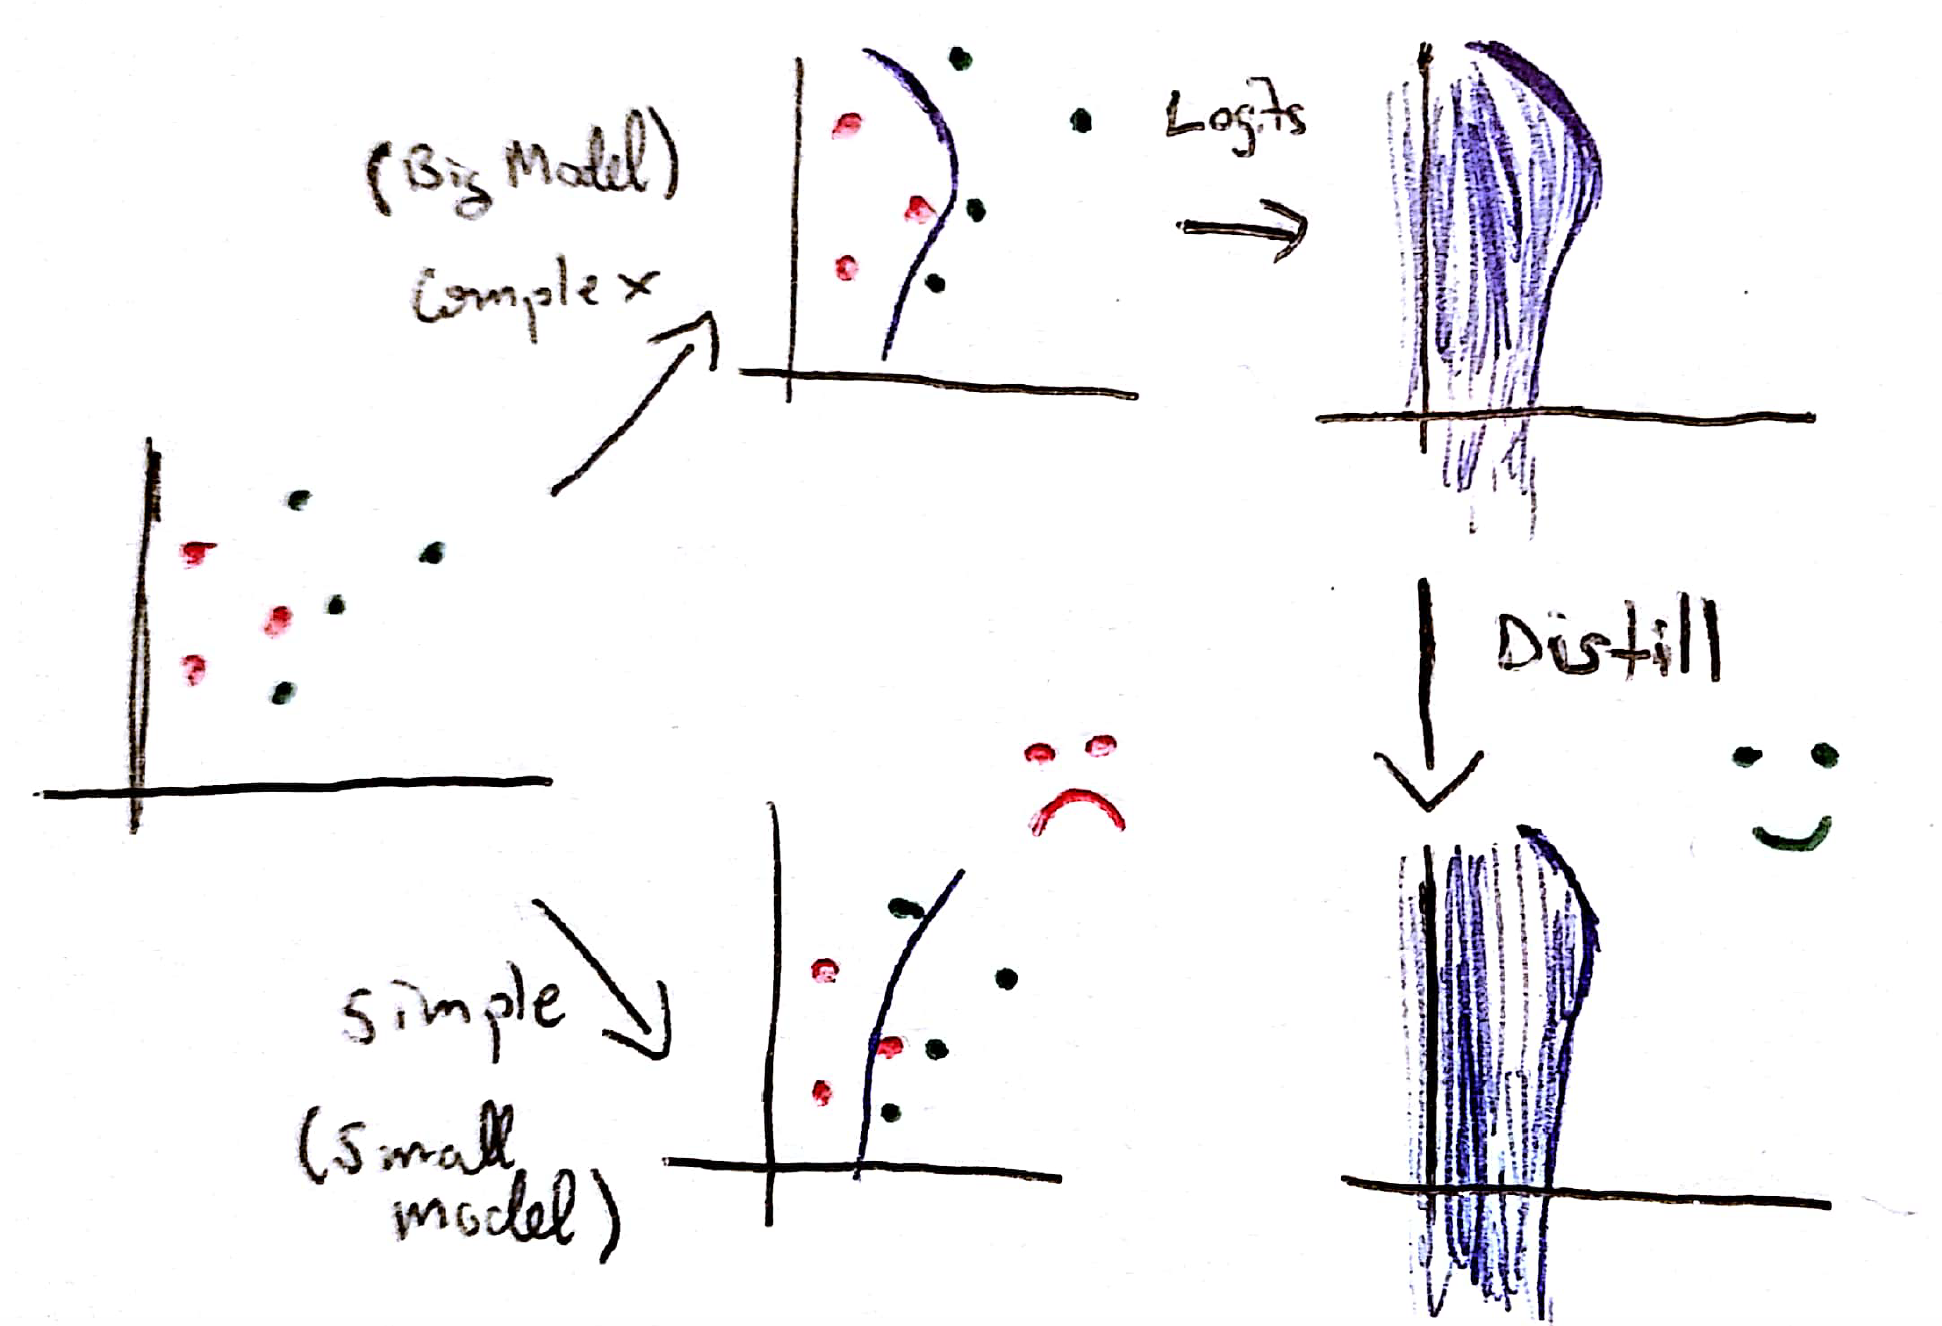
\includegraphics[width=0.45\paperwidth]{figure/distillation_overview}
  \caption{Distilling a complex model to a simple model class often works better
    than attempting to directly learn within the simple model
    class. \label{fig:distillation_overview} }
\end{figure}
\end{frame}

\begin{frame}
  \frametitle{Distillation by Trees}
  \begin{itemize}
  \item Proposal: Approximate teacher logits by class of soft decision trees
    \begin{itemize}
    \item Branching probabilities at node $i$: $\sigma\left(x^{T}w_i +
      b_i\right)$
    \item Internal nodes still learn filters $w_i$
    \item But now can inspect paths for each decision
    \end{itemize}
  \end{itemize}
\begin{figure}[ht]
  \centering
  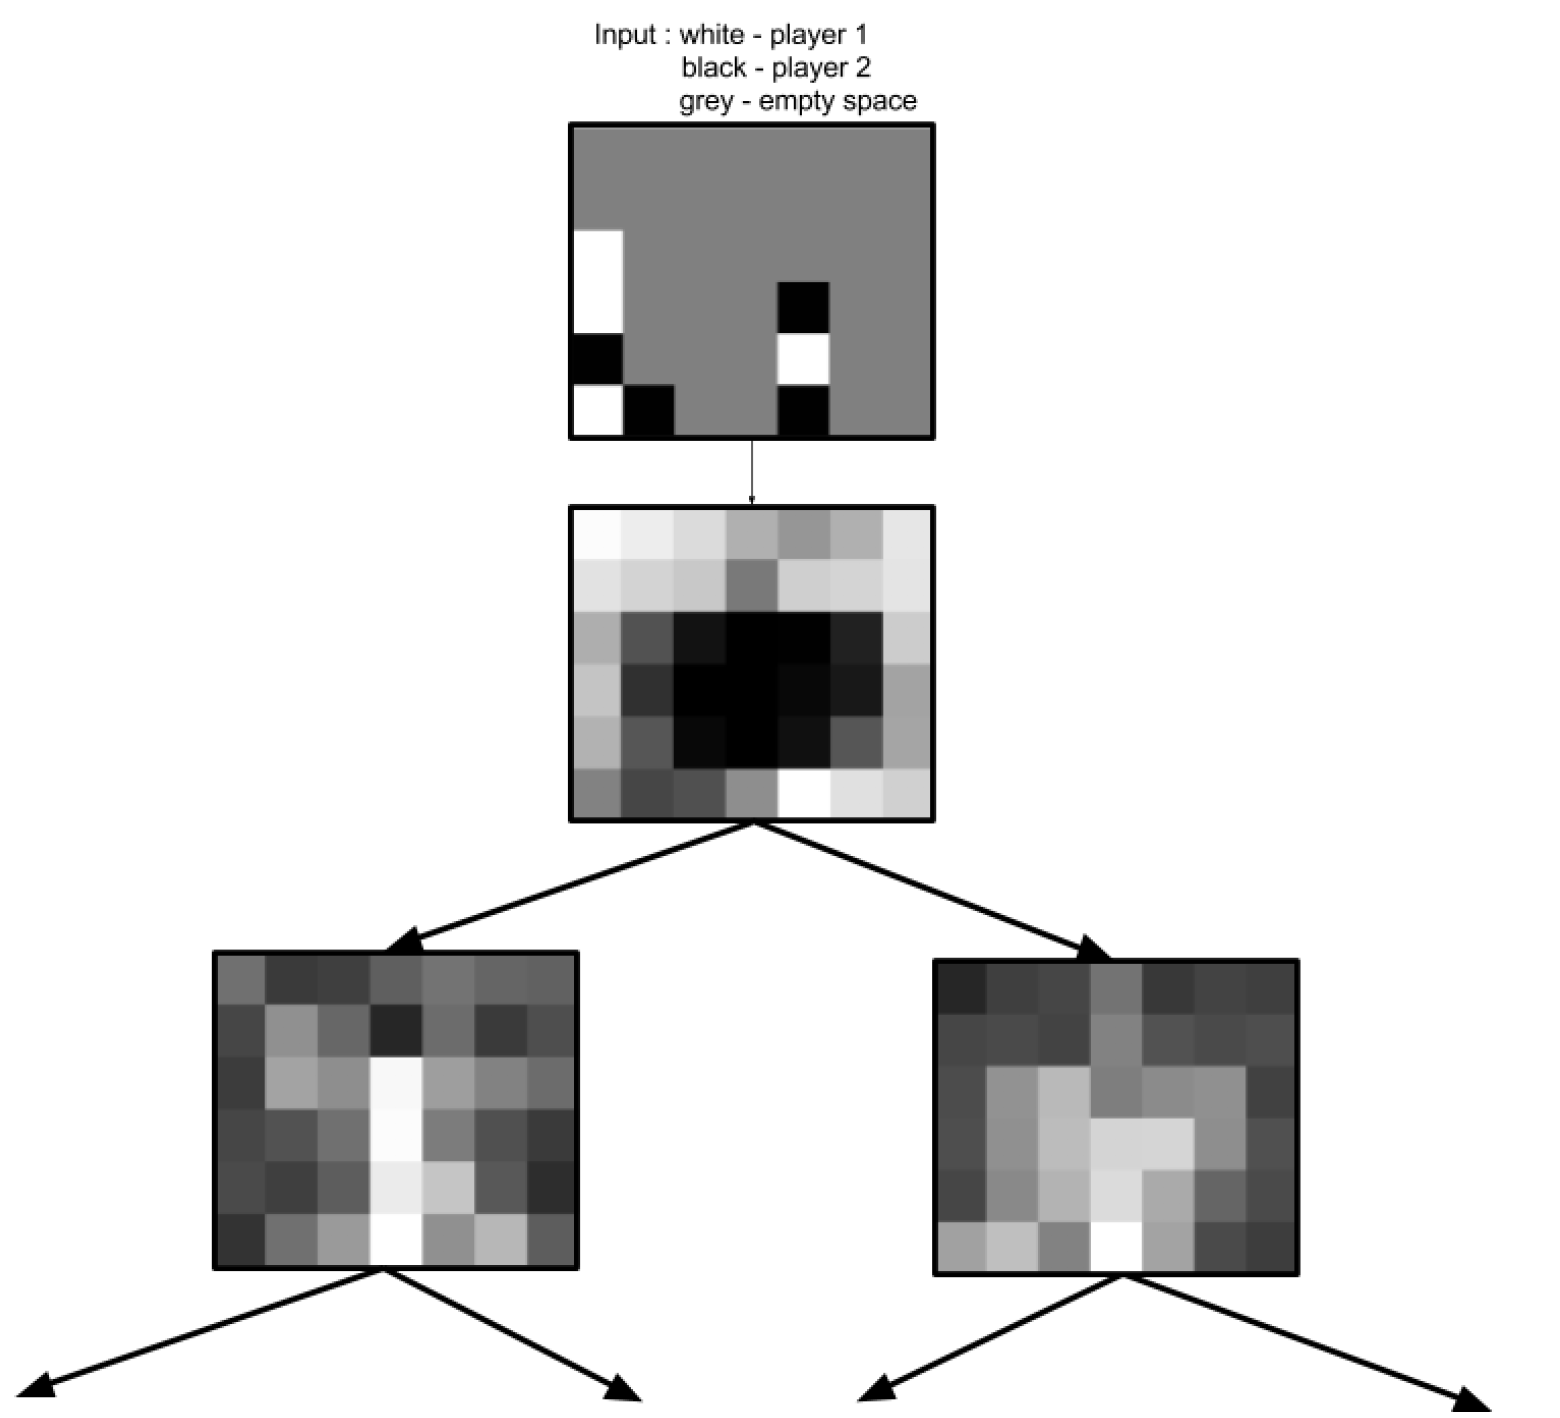
\includegraphics[width=0.4\paperwidth]{figure/connect4}
  \caption{It's possible to inpsect learned features at decision nodes, as in
    this Connect 4 example. \label{fig:connect4} }
\end{figure}

\end{frame}

\begin{frame}
  \frametitle{Additive Models}
  \begin{itemize}
  \item Approximate regression / decision surface by additive model with
    interactions
    \begin{itemize}
    \item $F\left(x\right) = b_0 + \sum h_{j} \left(x_j\right) + \sum_{j \neq k} h_{jk}\left(x_{j}, x_{k}\right) + \dots$
    \end{itemize}
  \item Can directly inspect changes in predictions when changing values of
    specific features
  \item Good for tabular data
  \item Bad when features need to be learned from raw inputs
  \end{itemize}
\end{frame}

\begin{frame}
  \frametitle{Additive Models}
 \begin{figure}[ht]
   \centering
   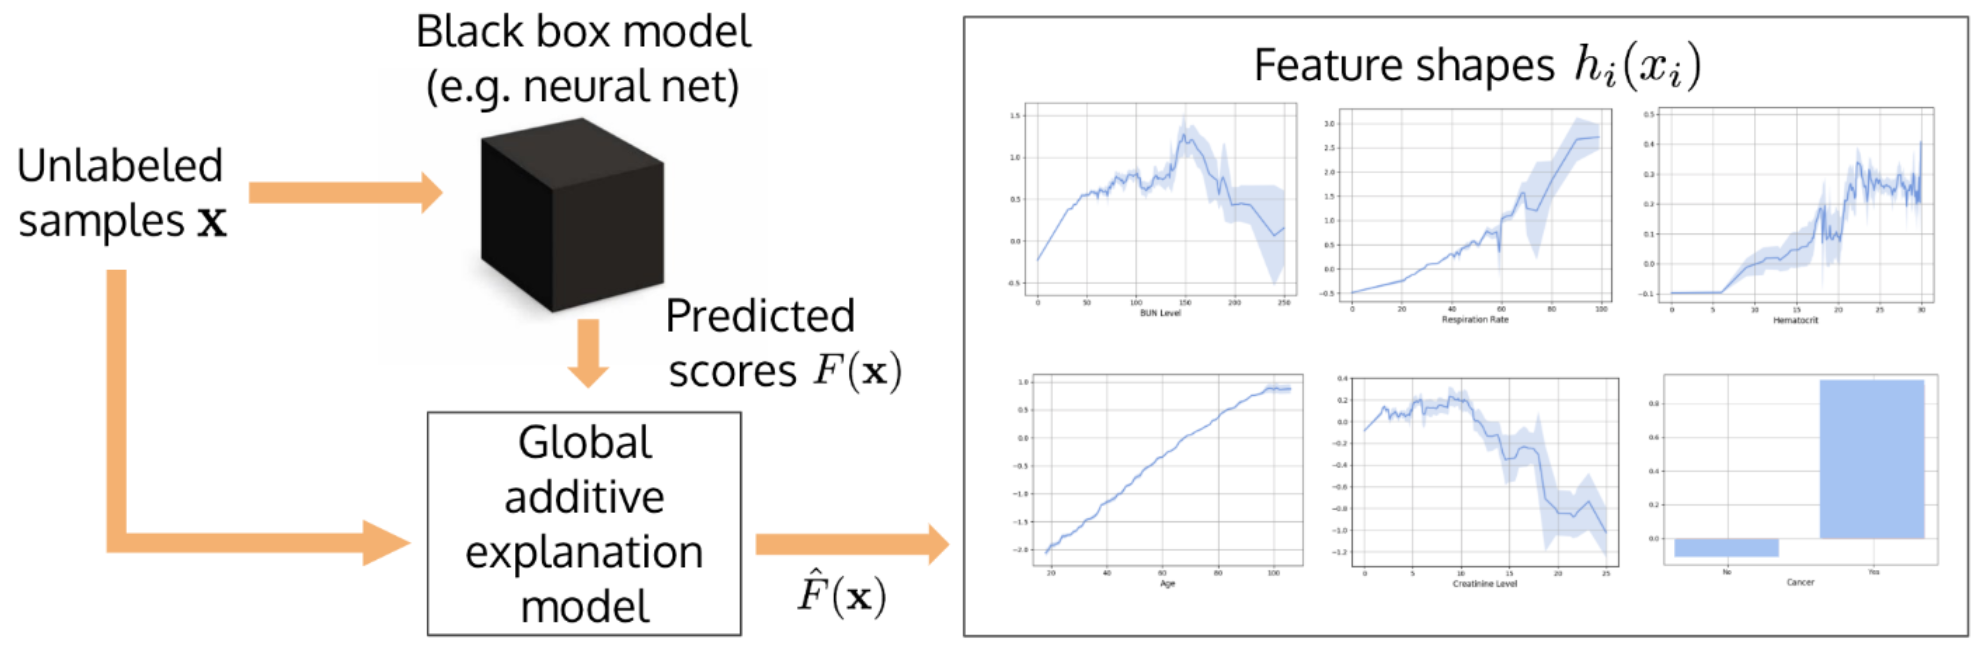
\includegraphics[width=0.7\paperwidth]{figure/additive}
   \caption{Example first-order additive features learned by
     distillation. \label{fig:additive} }
 \end{figure}
\end{frame}

\section{Perturbations}

\begin{frame}
  \frametitle{Perturbations}
  \begin{itemize}
  \item Intentional perturbation can be illuminating
  \item What happens when you change...
    \begin{itemize}
    \item Raw pixel values?
    \item Presence of training example?
    \item Layer activation values?
    \end{itemize}
  \end{itemize} 
\end{frame}

\begin{frame}
  \frametitle{Saliency Maps}
  \begin{itemize}
  \item For a given image, how would class predictions change if you manipulated
    a pixel?
  \item Simplest version: $\nabla_{x} f_{\theta}\left(x\right)$ change in class
    given infinitesimal changes in inputs
  \end{itemize} 
\begin{figure}[ht]
  \centering
  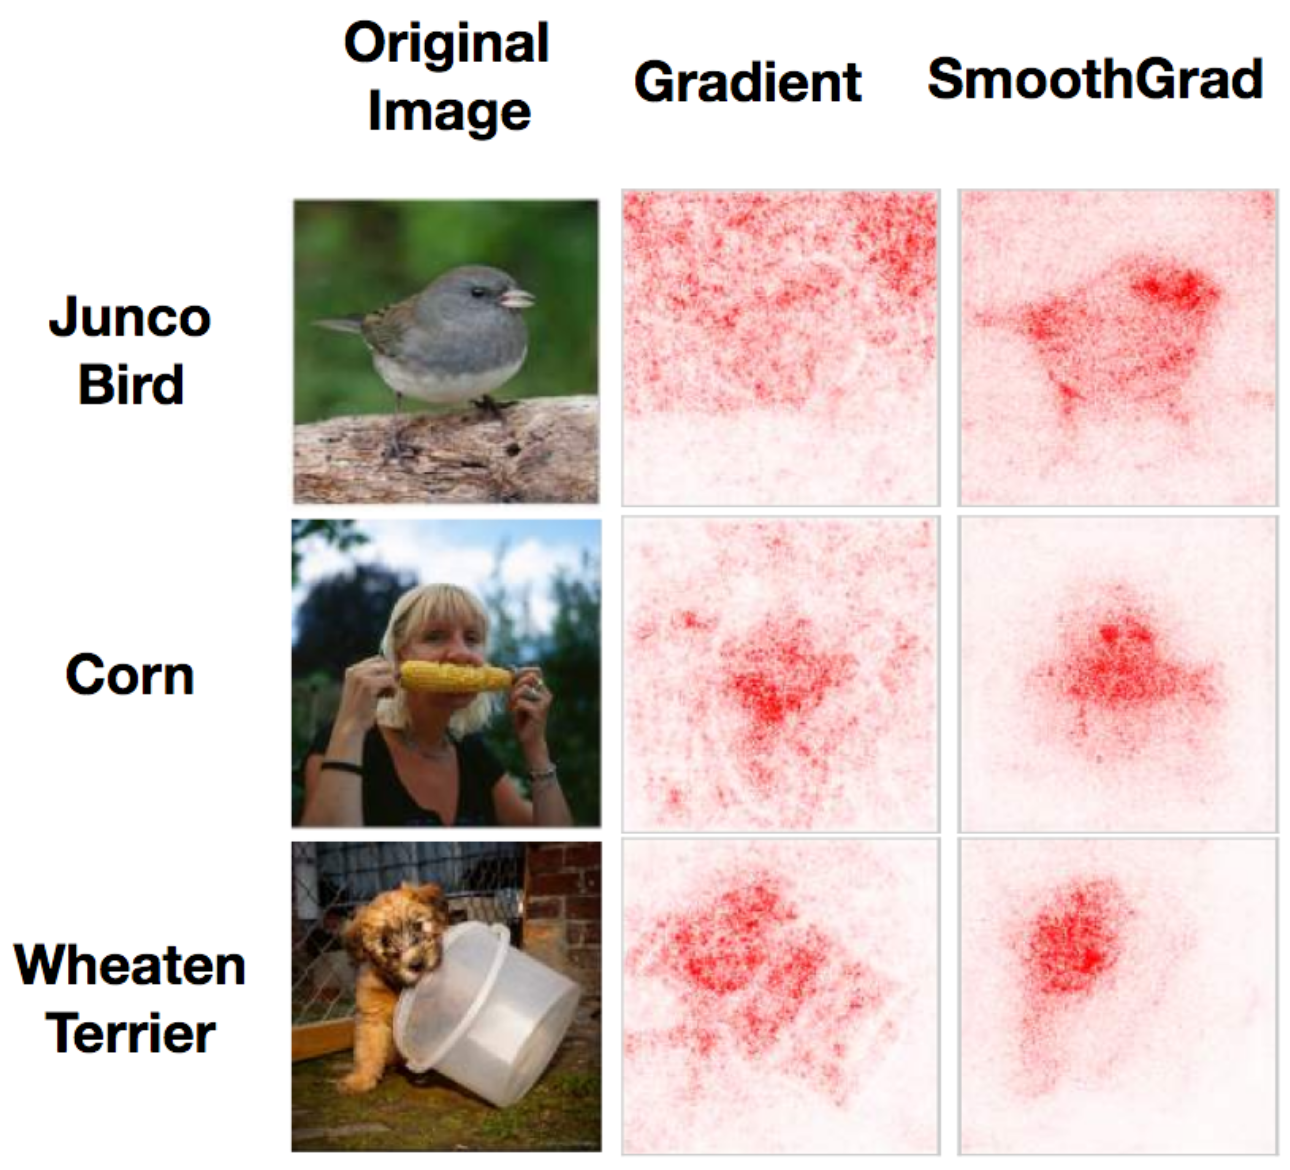
\includegraphics[width=0.4\paperwidth]{figure/saliency}
  \caption{Example saliency maps. Smooth-grad just averages the gradient map
    over many noisy versions of input image.\label{fig:saliency} }
\end{figure}
\end{frame}

\begin{frame}
  \frametitle{Cautionary advice...}
 \begin{itemize}
 \item While simple to implement, use cases aren't entirely clear
 \item Still have to inspect one example at a time
 \item Many proposals don't pass \textit{sanity checks}
 \end{itemize} 
\end{frame}

\subsection{Influence Functions}

\begin{frame}
  \frametitle{Influence Functions}
  \begin{itemize}
  \item Classical notion from statistics: Influential datapoints
  \item Measures sensitivity of fit to removal of points
  \end{itemize} 
  \begin{figure}[ht]
    \centering
    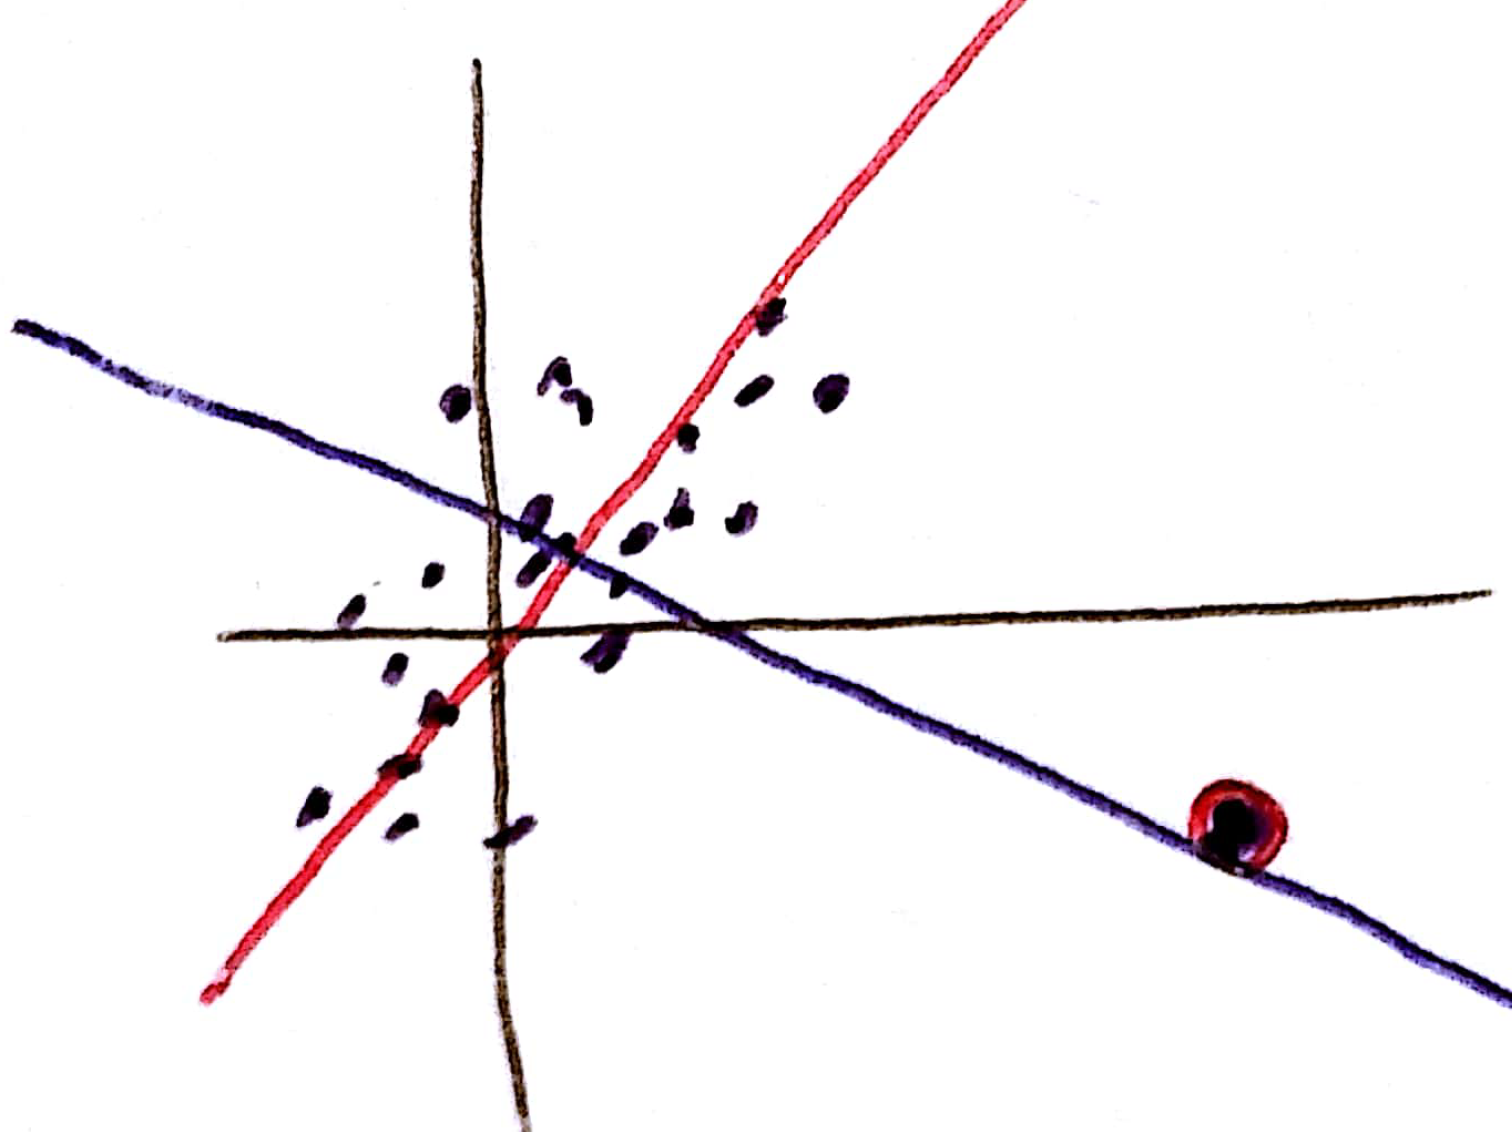
\includegraphics[width=0.7\paperwidth]{figure/classical_influence}
    \caption{The difference between fits when you include vs. remove a point is
      called that point's influence.\label{fig:classical_influence} }
\end{figure}
\end{frame}

\begin{frame}
  \frametitle{Contributions}
  \begin{itemize}
  \item Change in loss at (potentially new point) $z$ when $\eps$-upweight
    training pair $z_i = \left(x_i, y_i\right)$
    \begin{align*}
    I\left(z, z_i\right) = -\nabla_{\theta} \ell\left(z, \hat{\theta}\right)^{T} H^{-1}_{\hat{\theta}} \nabla_{\theta} \ell\left(z_i, \hat{\theta}\right)
    \end{align*}
  \item Alignment between gradients of loss at new and old points, after
    adjusting for local curvature 
    \begin{itemize}
    \item More alignment $\rightarrow$ larger decrease in loss
    \end{itemize}
  \item Applied of SGD-able approximations to Hessian $H^{-1}_{\hat{\theta}}$
  \end{itemize}
\end{frame}

\begin{frame}
  \frametitle{Applications}
  \begin{itemize}
  \item Identifying most influential points for specific test cases
  \item Identifying mislabled points in training data
  \item Not restricted to deep learning!
  \end{itemize} 
\begin{figure}[ht]
  \centering
  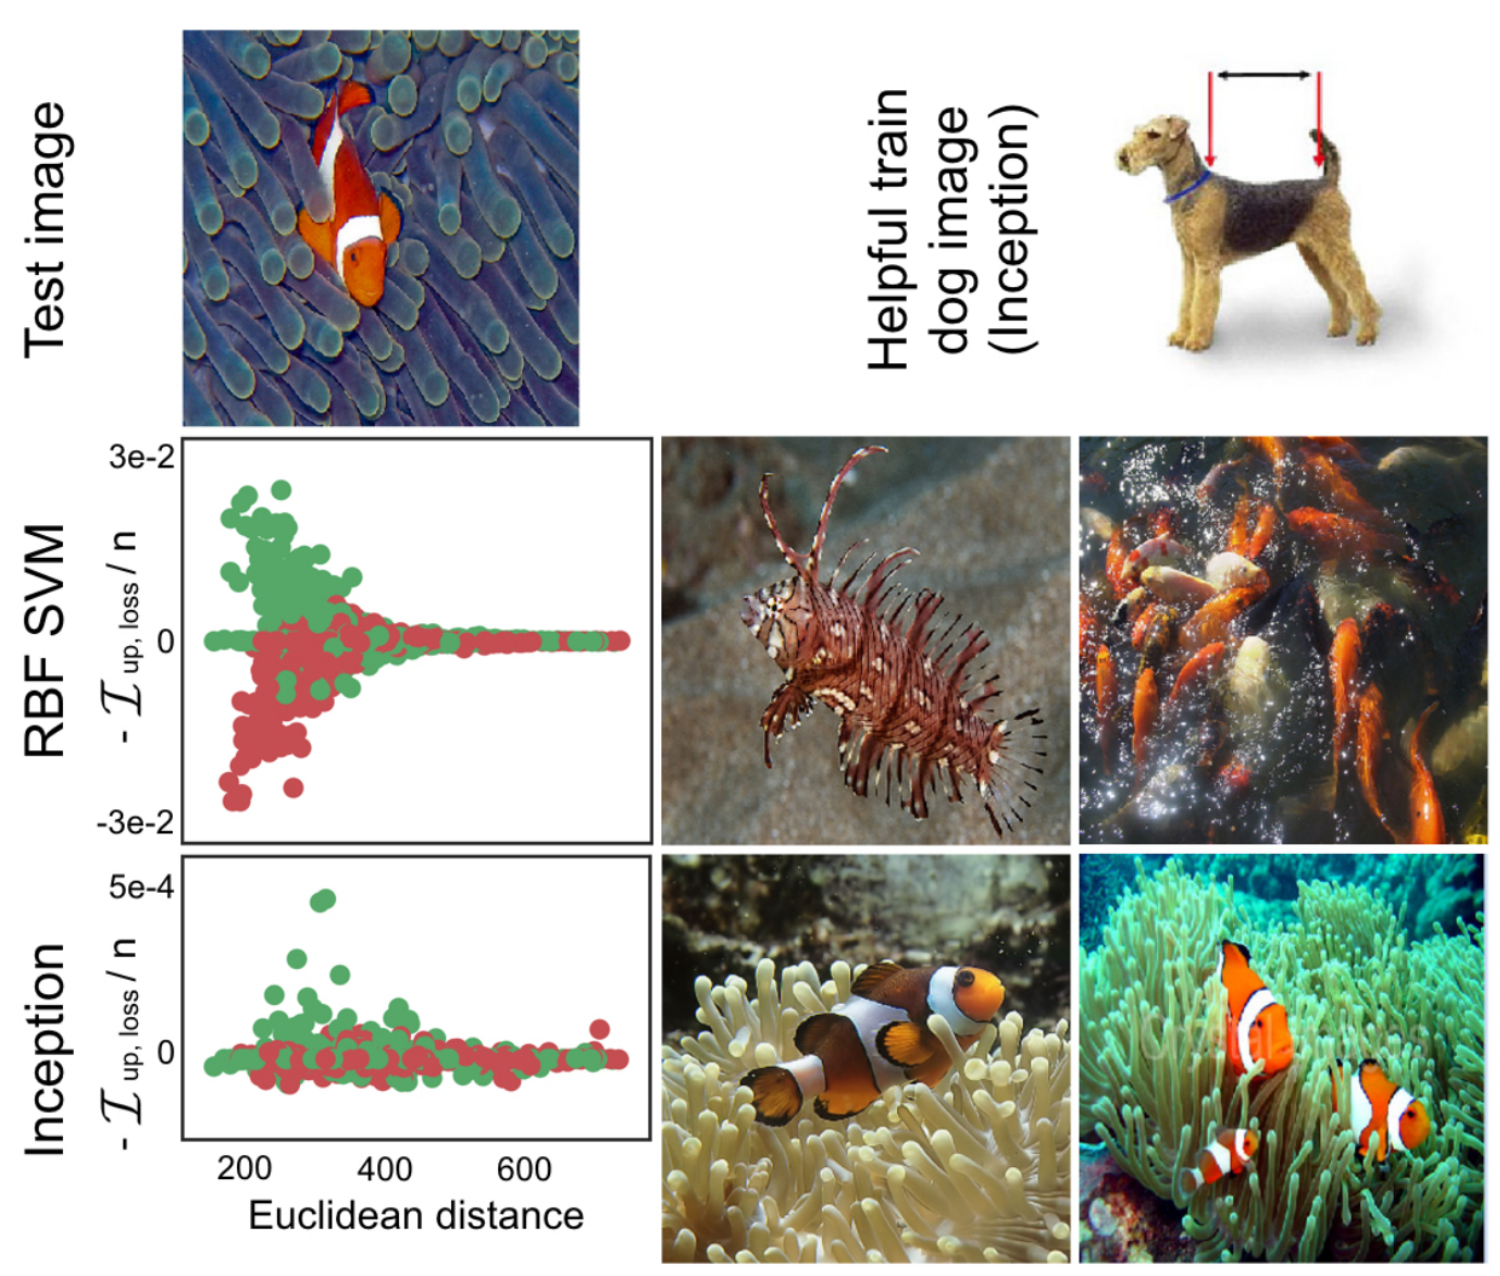
\includegraphics[width=0.45\paperwidth]{figure/influential}
  \caption{Example influential observations from \citep{koh2017understanding}\label{fig:influential}
  }
\end{figure}
\end{frame}

\subsection{Concept Activation Vectors}

\begin{frame}
  \frametitle{Concept Activation Vectors}
  \begin{itemize}
  \item What if you had a specific ``concept'' that you wanted to test model
    sensitivity to?
    \begin{itemize}
    \item Importance of anemone to predicting clownfish?
    \end{itemize}
  \item Need workable definition of a concept...
  \end{itemize}
\end{frame}

\begin{frame}
  \frametitle{Formulation}
  \begin{itemize}
  \item Idea: Have the user provide concepts!
  \item Study how concept affects feature activations, one layer at a time
  \end{itemize} 
\end{frame}

\begin{frame}
  \frametitle{User concepts}
  \begin{itemize}
  \item User creates set of ``concept'' samples (or chooses them from a
    database, using image tags, say)
  \item Create activations $f_{l}$ at layer $l$ for both concept and random
    nonconcept examples
  \item Define concept activation $v_{C}^l$ based on learned linear decision
    boundary
  \end{itemize} 
  \begin{figure}[ht]
    \centering
    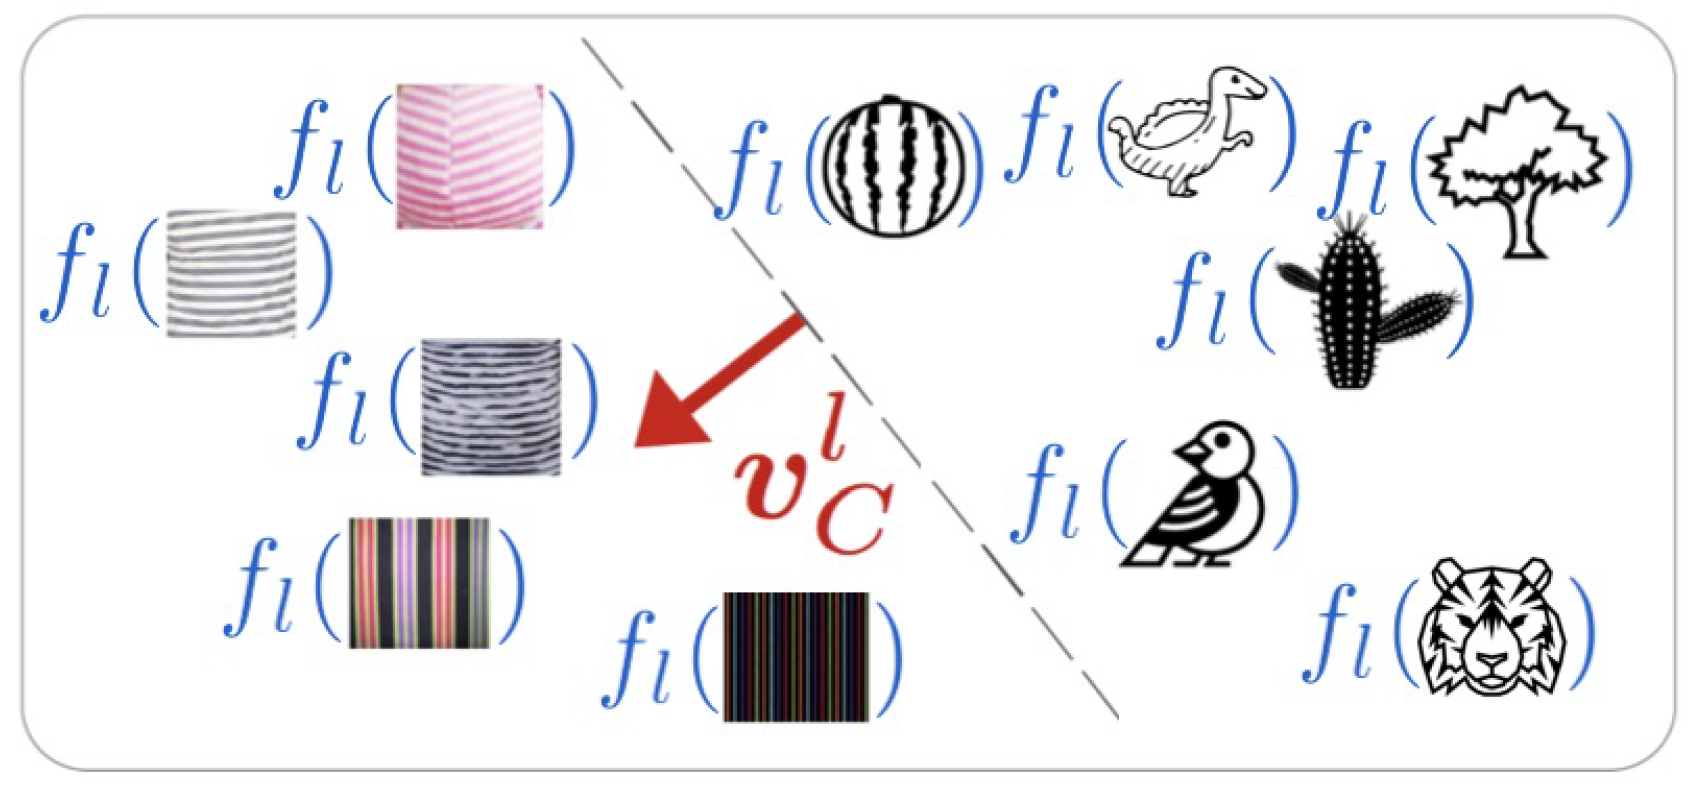
\includegraphics[width=0.6\paperwidth]{figure/cav_space}
    \caption{The CAV vector is defined as the direction that separates samples
      representative of a concept (like stripes) and unrelated random samples.
      \label{fig:cav_space} }
  \end{figure}
\end{frame}

\begin{frame}
  \frametitle{Effect of Concepts}
  \begin{itemize}
  \item See how logit $h_{lk}$ changes when nudging layer $l$ activations
    $f_{l}\left(x\right)$ for example $x$ towards concept $C$
    \begin{align*}
      S_{k, C, l}\left(x\right) &= \lim_{\eps \downarrow 0} \frac{h_{lk}\left(f_{l}\left(x\right) + \eps v_{C}^l\right) - h_{lk}\left(f_l\left(x\right)\right)}{\eps}
    \end{align*} 
  \item Averaging this over examples $x$ from class of interest
  \end{itemize} 
\begin{figure}[ht]
  \centering
  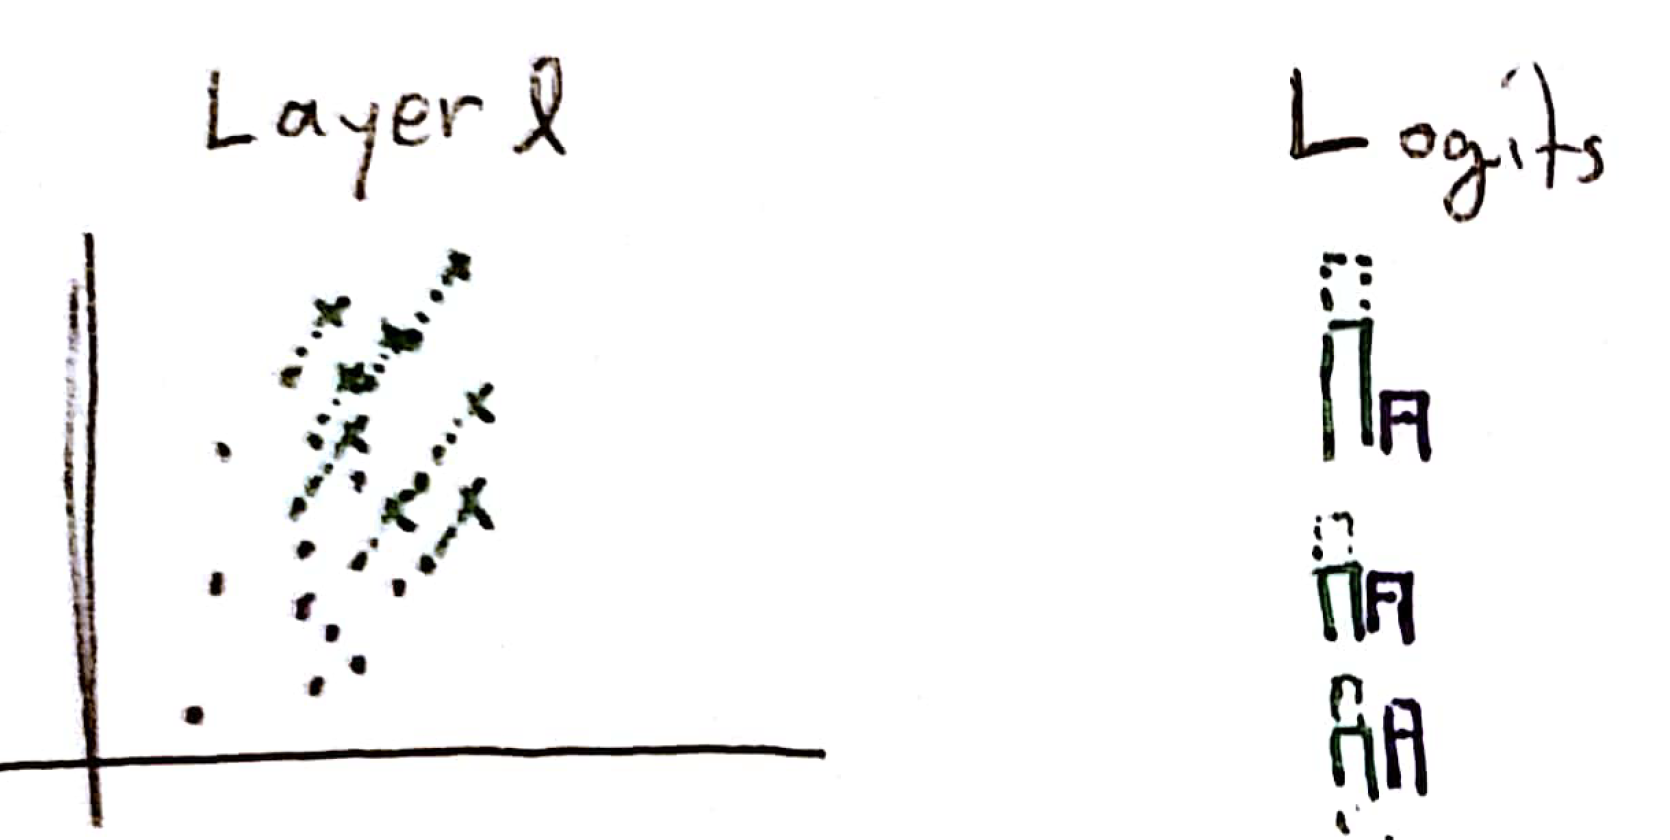
\includegraphics[width=0.6\paperwidth]{figure/cav_derivs}
  \caption{The CAV score for a class is the amount the logit for that class
    changes in response to perturbing its examples in the CAV
    direction. \label{fig:cav_derivs} }
\end{figure}
\end{frame}

\begin{frame}
  \frametitle{Applications}
  \begin{itemize}
  \item Find examples within a class most and least similar to specified concept
    \begin{figure}[ht]
      \centering
      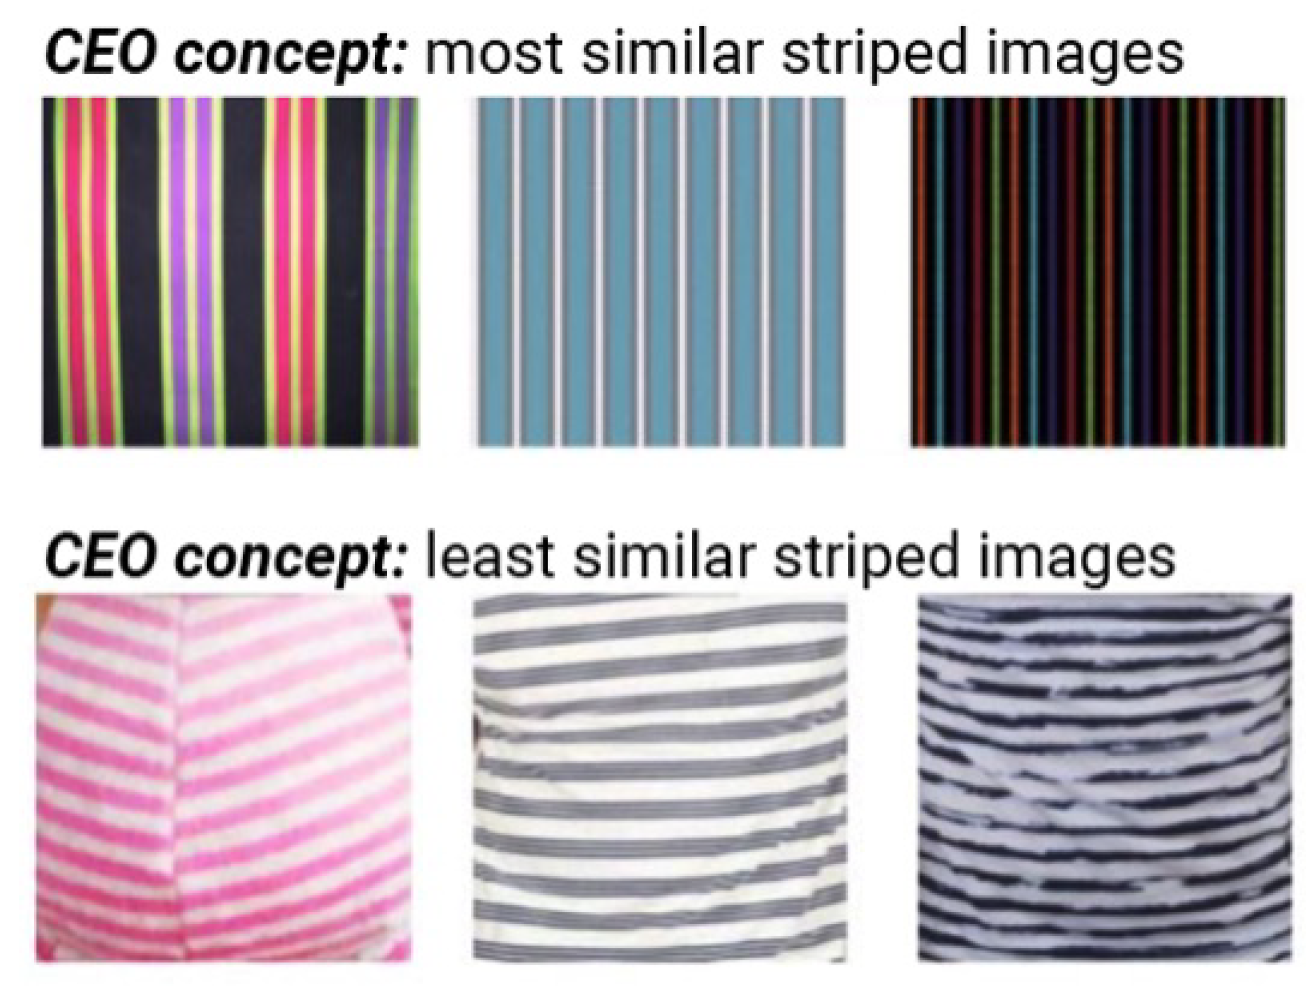
\includegraphics[width=0.7\paperwidth]{figure/cav_app3}
    \end{figure}
  \end{itemize}  
\end{frame}

\begin{frame}
  \frametitle{Applications}
  \begin{itemize}
  \item Quantify potential sources of bias
    \begin{figure}[ht]
      \centering
      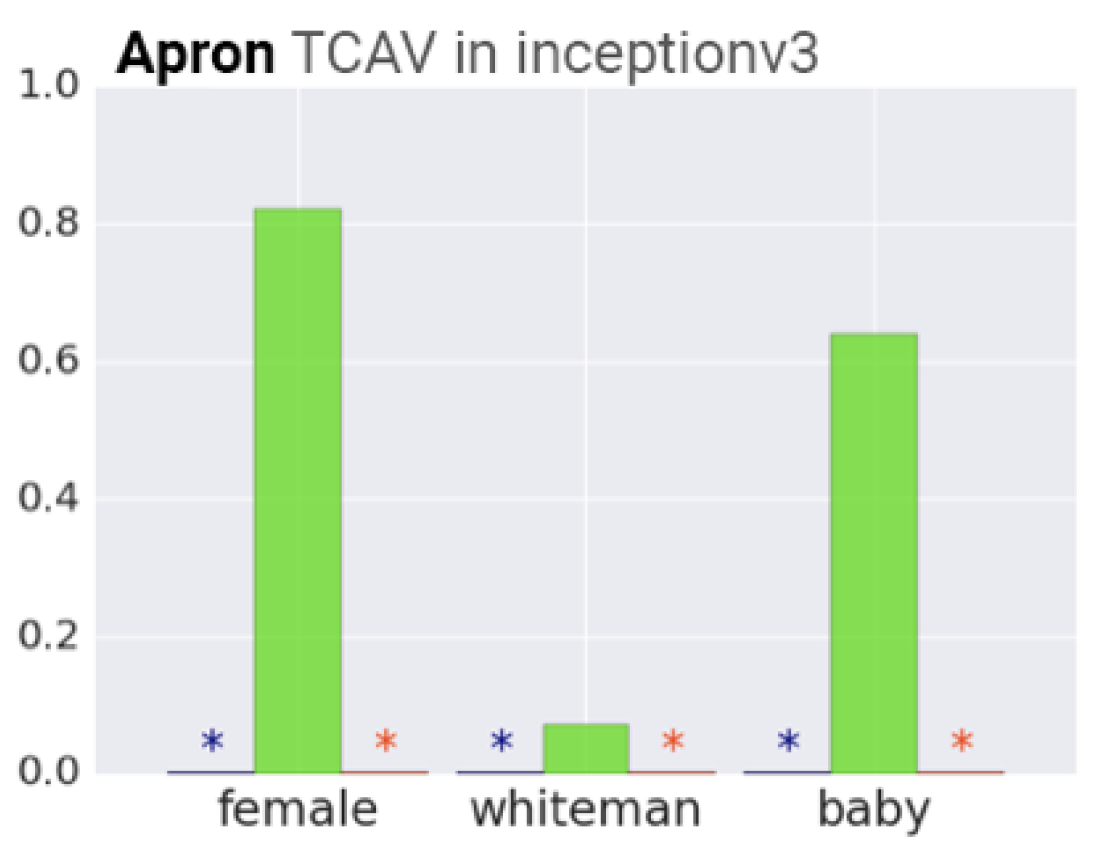
\includegraphics[width=0.7\paperwidth]{figure/cav_app2}
    \end{figure}
  \end{itemize}  
\end{frame}

\begin{frame}
  \frametitle{Applications}
  \begin{itemize}
  \item Measuring consistency with codified medical practice
    \begin{figure}[ht]
      \centering
      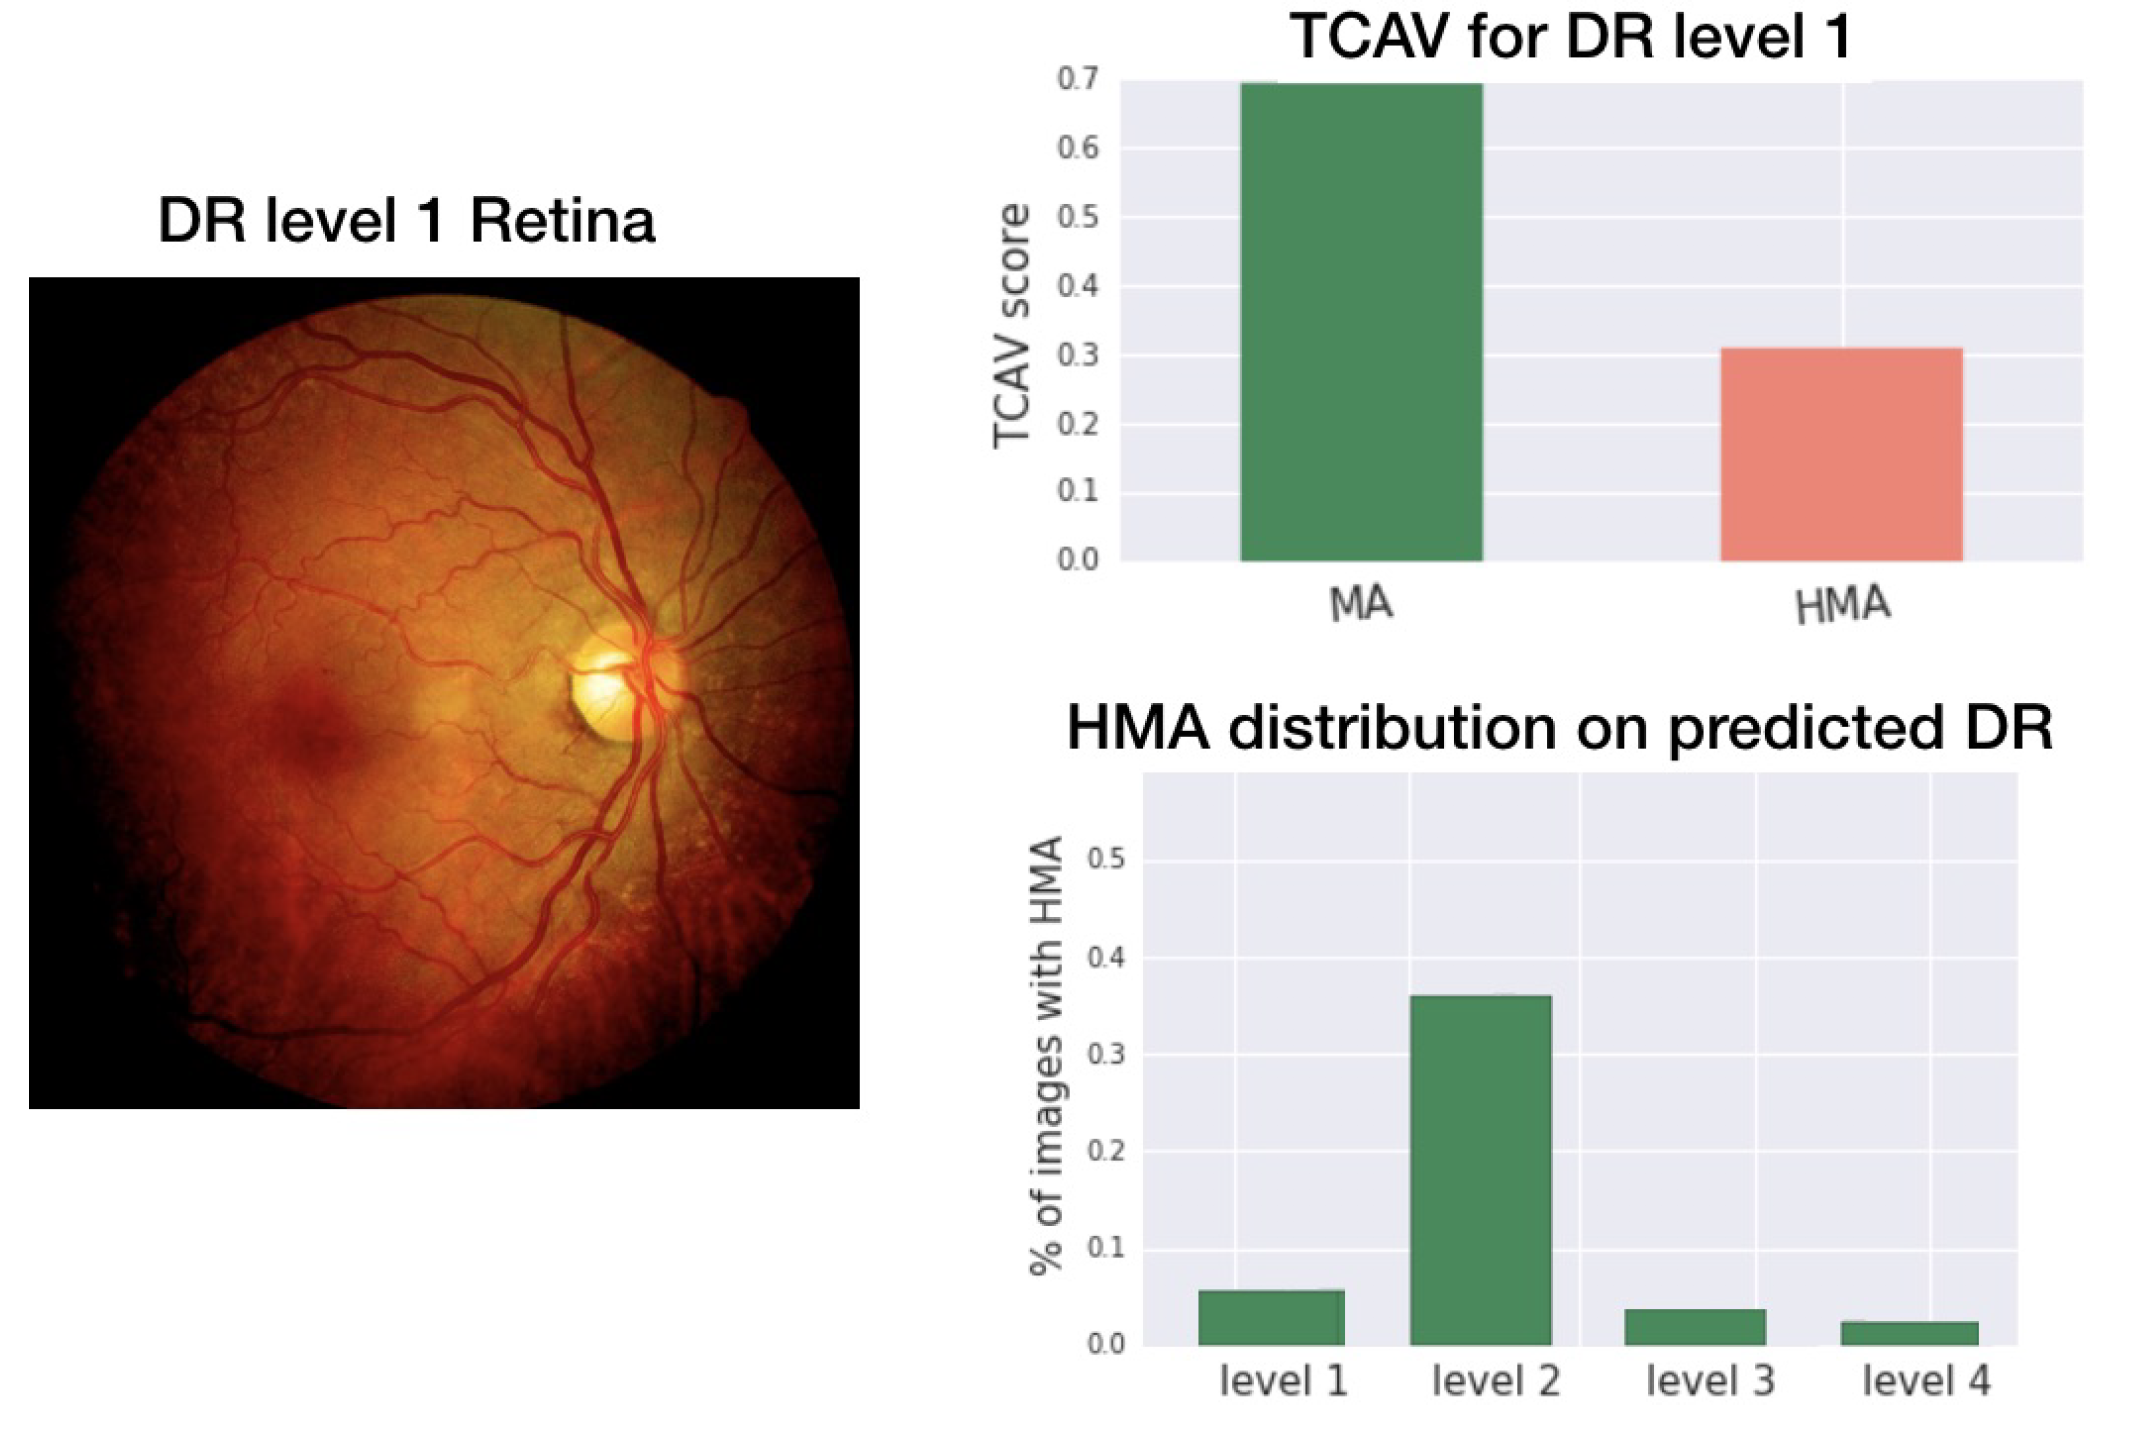
\includegraphics[width=0.7\paperwidth]{figure/cav_app1}
    \end{figure}
  \end{itemize}  
\end{frame}

\begin{frame}
  \frametitle{Conclusion}
\begin{itemize}
\item As complicated as it can be to interpret models... still usually simpler
  than interpreting people
\end{itemize}
\end{frame}

\end{document}
